\documentclass[conference]{IEEEtran}
\IEEEoverridecommandlockouts
% The preceding line is only needed to identify funding in the first footnote. If that is unneeded, please comment it out.
\usepackage{cite}
\usepackage{amsmath,amssymb,amsfonts}
\usepackage{algorithmic}
\usepackage{graphicx}
\usepackage{wrapfig}
\usepackage{textcomp}
\usepackage{xcolor}
\usepackage{booktabs}
\usepackage{siunitx}
\graphicspath{{figures/}}
\def\BibTeX{{\rm B\kern-.05em{\sc i\kern-.025em b}\kern-.08em
    T\kern-.1667em\lower.7ex\hbox{E}\kern-.125emX}}
\begin{document}

\title{EECS 470}

\author{Jiahe Ding, Hongzheng Hu, Qijia Liu, Junde Song, Junwen Yu, Kangqi Zhang
}

\maketitle

\begin{abstract}
This report presents our design and performance analysis of an out-of-order RISC-V processor using SystemVerilog, based on the MIPS R10K architecture. The processor integrates advanced features such as n-way superscalar, ETB, EBR, and other local features. Key optimizations include changing the width of CDB and the size of all kinds of modules. Also, we experiment on branch prediction strategies and cache associativities. Finally, our design reaches a clock period of 10ns and an average CPI of 1.68. For testing and verification, we mainly built a cycle-accurate simulator in C++ to help us debug. 
\end{abstract}

\begin{IEEEkeywords}
MIPS R10K, Out-of-order processor, EECS 470
\end{IEEEkeywords}

\section{Introduction}

This report presents a SystemVerilog-based processor design supporting out-of-order execution and full compliance with the RISC-V specification. Our objective is to have the program time cost as short as possible. This can be divided into 2 parts: CPI and clock period, both of which should be as small as possible. 

The report is organized as follows: First, we detail the micro-architecture design. Subsequently, we show results including program-specific runtime performance and the clock period. Following this, we conduct data-driven analysis of design tradeoffs and possible improvements. Then, we mention our verification and testing methodologies. Finally, we outline how our group is collaborating to reach this result.

\section{Project Design}
In this project, we've implemented an N-way MIPS R10K architecture. It mainly includes a register renaming technique. All registers will be renamed into a tag in the Physical Register File(PRF) when they are dispatched. This can help avoid data hazards. The detailed module layout can be found in Fig. \ref{fig:high_level}.

\begin{figure}[htbp]
\centerline{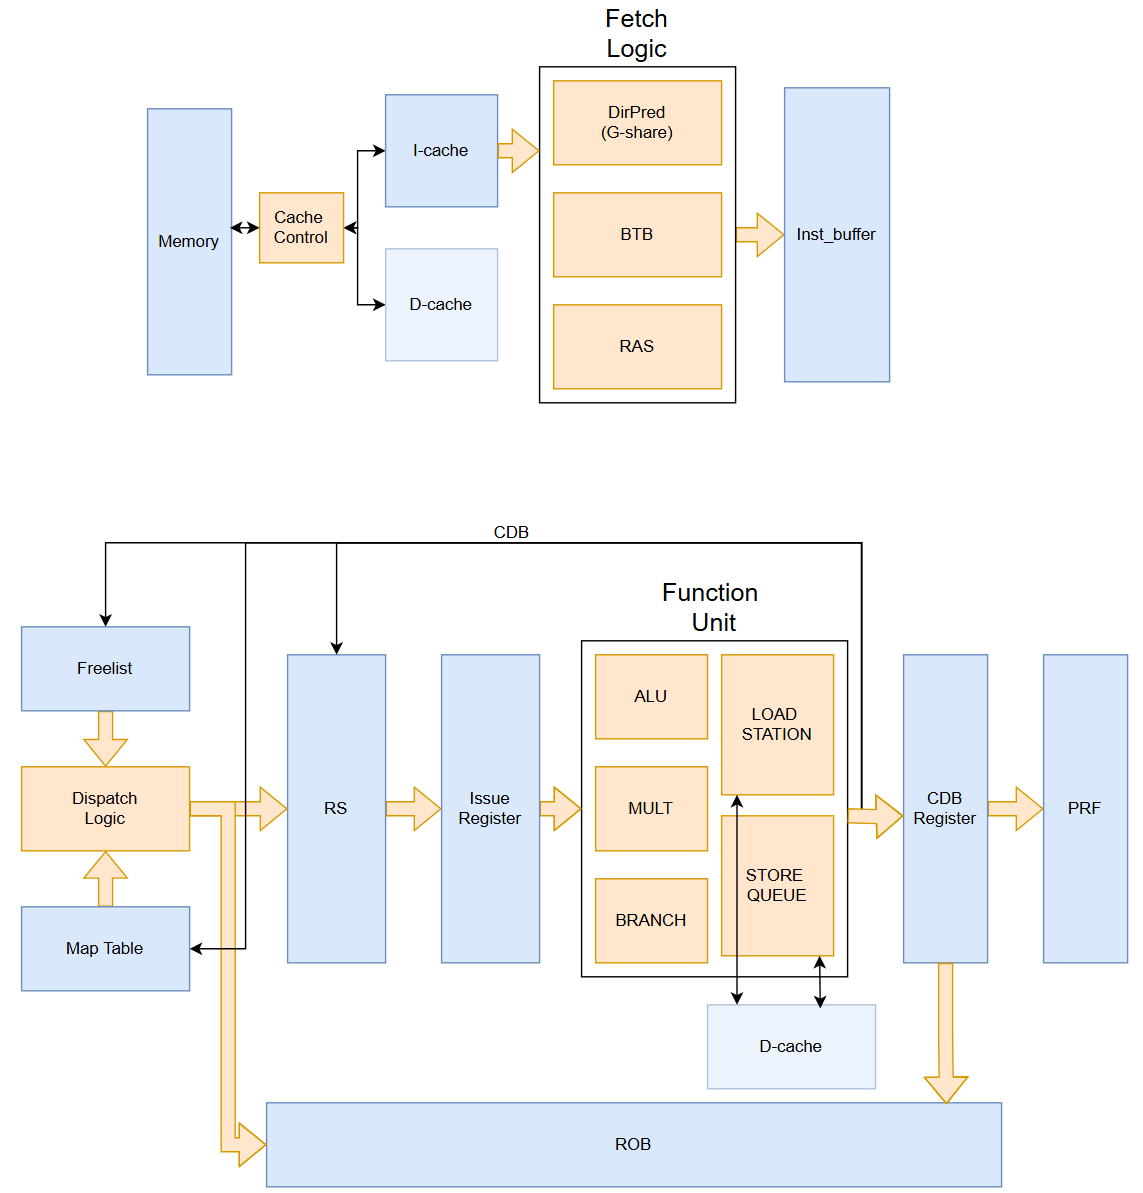
\includegraphics[width=0.3\textwidth]{figures/overall.png}}
\caption{High-level design.}
\label{fig:high_level}
\end{figure}


In the diagram, blue blocks represent registers and orange ones represent combination logic. Meanwhile, we've also implemented other advanced features. 

\subsection{List of Features}

\subsubsection{Features Present in the Final Design}

\begin{itemize}
  \item N-way superscalar
  \item Early Branch Resolution
  \item Early Tag Broadcast
  \item G-Share Branch Predictor
  \item Return Address Stack
  \item Instruction Prefetching
  \item Dual-ported, banked i-cache
  \item Non-blocking d-cache
  \item Out-of-order issue of mem requests (loads)
  \item Data forwarding from stores to loads
  \item Testing \& Debugger: see corresponding sections
\end{itemize}

\subsubsection{Features not in the Final Design}

We made explorations in various directions. Some features are not incorporated in our final submission, either due to performance reasons or time constraints. Here is a list of them, and where to find them:

\begin{itemize}
  \item Advanced Predictors: TAGE-like, Perceptron, and CNN. Implemented on branch "bp-TAGE2" (TAGE-like), branch "bp-CNN" (1-layer CNN), branch "bp-n-layer-CNN" (n-layer CNN), and "perception" (perceptron, note the typo in branch name), file "verilog/dirPred.sv"
  \item Associative d-cache. Implemented on branch "associative\_cache" (2-way) and "fourway" (4-way), file "verilog/dcache.sv"
  \item Issuing instructions in program order. Implemented on branch "rs-age-logic", file "verilog/rs.sv"
\end{itemize}

\subsection{Basic Components}
\subsubsection{Reservation Station}

We've designed a 16-entry Reservation Station (RS). It will receive the instruction from dispatch and record the new tag designated by Free List. Also, it will keep updating the readiness of the source tag from Common Data Bus (CDB) in order to prevent the read after write (RAW) problem. 

Meanwhile, it will issue the instruction that has all source registers ready to the Issue Register and Function Units. 

\subsubsection{Re-Order Buffer}

Our Re-Order Buffer (ROB) is a 32-entry FIFO table. It has two pointers of head and tail, to keep track of the FIFO list. During the dispatch stage, every instruction will be allocated at the end of the list in ROB. Every instruction will be marked complete when it leaves the complete stage. Since we want to seek a precise state, instructions are retired in order. ROB will send the old tag of that instruction to Free List to recycle it. 

\subsubsection{Freelist and maptable}

These two modules are used to keep track of the register renaming state. We have 64 tags and PRF in total. Free List is to keep the unused tags and allocate these tags to the newly dispatched instructions. It also recycles the old tags of retired instructions. Map Table records the mapping of architecture register with the tag. It will also keep track of the readiness of each tag. Once receives a tag in the CDB, it will mark that tag as ready. 

\subsubsection{Function Units}

We totally have 3 ALUs, one 4-stage mult unit, one branch unit, one load unit, and one store unit. Mult unit is responsible for all multiplication instructions and ALUs for other arithmetic instructions. Branch unit contains a comparator to resolve the branch result and an adder to calculate the target PC. It is also where JAL and JALR instructions go. Load unit and store unit both contain one adder, which is responsible for calculating the memory address they want to access. These results will be sent to load station and store queue for further processing. 


\subsection{ETB}
Because of the limited width of Common Data Bus, after leaving the execute stage, all calculated results will be written into to CDB register, waiting for arbitration. In the next cycle, the arbiter will choose several to get into the CDB and write back to the PRF. The CDB contains the tag that has finished writing back. 

However, with ETB feature, the arbitration will happen one cycle early, and the tag will be broadcast one cycle early. For one stage units (ALU, branch and store unit), they will run for the CDB. If they succeed, they will be issued. If not, they will still stall in the RS instead of the execution stage. Meanwhile, mult unit will be running for CDB one cycle earlier (i.e. last but one stage) and will only continue to final stage if it is granted by CDB arbiter. As a result, we need to bypass the data in CDB reg to the issue stage. 

\subsection{Early Branch Resolution (EBR)}
In the basic pipeline design, branch instructions are resolved during the retire stage. If a branch instruction is found to have been mispredicted, all subsequent instructions in the pipeline are flushed, and the processor begins fetching from the correct target address. However, the outcome of a branch can be known as early as the execution stage. Resolving branches immediately after execution reduces the performance cost of mispredictions and improves overall throughput. This technique is referred to as Early Branch Resolution (EBR) in our design.

Because instructions are issued out of order, both preceding and succeeding instructions relative to the resolved branch can be present in the pipeline. To manage this, each instruction is tagged with a branch index, indicating its dependency on unresolved branches. This allows the system to selectively squash only the instructions along the mispredicted path, while preserving those that precede the branch in program order.

When a branch instruction is fetched, an entry in the branch stack is allocated, and the index of this entry is used as its branch index (b-index). Each instruction is also assigned a branch mask (b-mask), which records the indices of all currently unresolved branches. This mechanism is illustrated in Fig. \ref{EBR-fetch}.

\begin{figure}[htbp]
\centerline{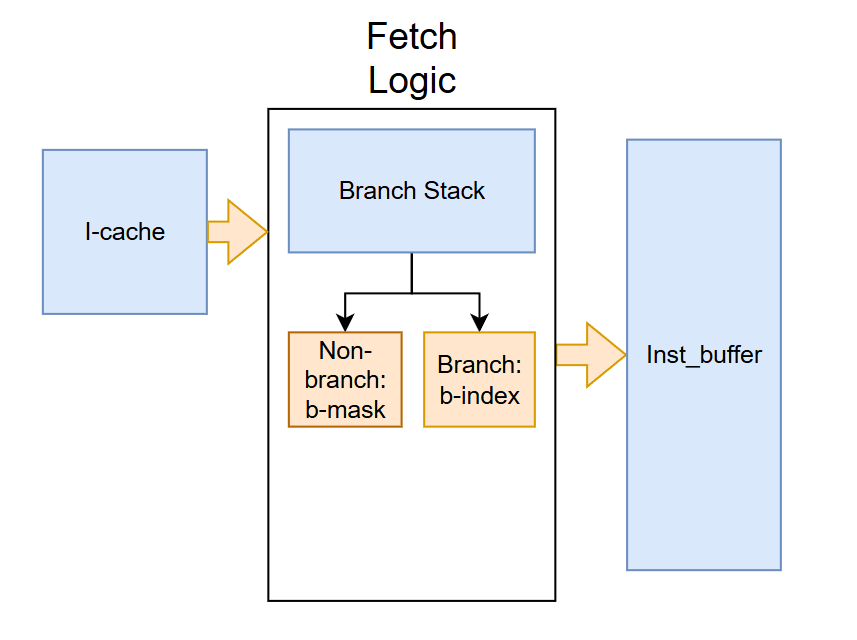
\includegraphics[width=0.6\columnwidth]{Design/EBR-fetch}}
\caption{Marking instructions with EBR logic. }
\label{EBR-fetch}
\end{figure}

When a branch is resolved, its outcome—whether the prediction was correct—and its branch index are broadcast to all pipeline stages holding instructions. If it was a misprediction, all instructions with the corresponding index in their b-mask are squashed. If the prediction was correct, the corresponding index is cleared from each instruction’s b-mask, indicating they no longer depend on that branch.

\subsection{N-Way Superscalar Design}
In a traditional 5-stage pipeline, each stage handles at most one instruction per cycle. To increase throughput, our processor adopts a superscalar architecture, which allows multiple instructions to progress through each stage simultaneously. We implement an N-way superscalar design, where N parameterizes the maximum number of instructions per stage.

In ideal conditions, when there are no inter-instruction dependencies, performance can theoretically scale by a factor of N. This approach boosts instruction-level parallelism and enhances overall processor efficiency.


\subsection{Cache}
Accessing main memory in our design incurs a 100ns latency. To mitigate this overhead, the processor employs caches that exploit spatial and temporal locality by storing recently accessed data. We implement separate caches for instructions and data, as their access patterns differ and exhibit minimal overlap.

\subsubsection{Instruction Cache}
The instruction cache (i-cache) is direct-mapped, banked, and supports prefetching. It is banked to enable parallel access to two memory blocks, supporting up to 4-way instruction fetch.

A stream buffer is employed to prefetch the next memory line while waiting for the current memory request to complete. The fetched data is temporarily stored in the stream buffer. If a requested address hits in the prefetch buffer, the corresponding block is deemed useful and promoted into the i-cache. If a request is made for an address not captured by the prefetch mechanism, the entire stream buffer is flushed, and prefetching resumes from the new address.

\subsubsection{Data Cache}
The data cache (d-cache) is a basic direct-mapped cache. It incorporates a Miss Status Holding Register (MSHR) to support non-blocking behavior. The MSHR stores requests that miss in the cache, allowing subsequent requests to proceed without stalling the pipeline. When the requested data is retrieved from memory, it is broadcast to fulfill the pending requests corresponding to that MSHR entry. This design enables the cache to issue useful memory requests every cycle without being bottlenecked by a single outstanding miss.

\subsection {Load Station and Store Queue}

Since the memory access has a long latency and withdrawing a memory write-back is quite hard, we need a store queue (SQ) that can monitor all store instructions before retire to keep the memory write-back in order. We also need a load station that can support out-of-order load issues and complete. Our strategy is non-speculative. You can see our design in Fig. \ref{fig:lsq}. SQ is a FIFO and load station is not in order. 

\begin{figure}[htbp]
\centerline{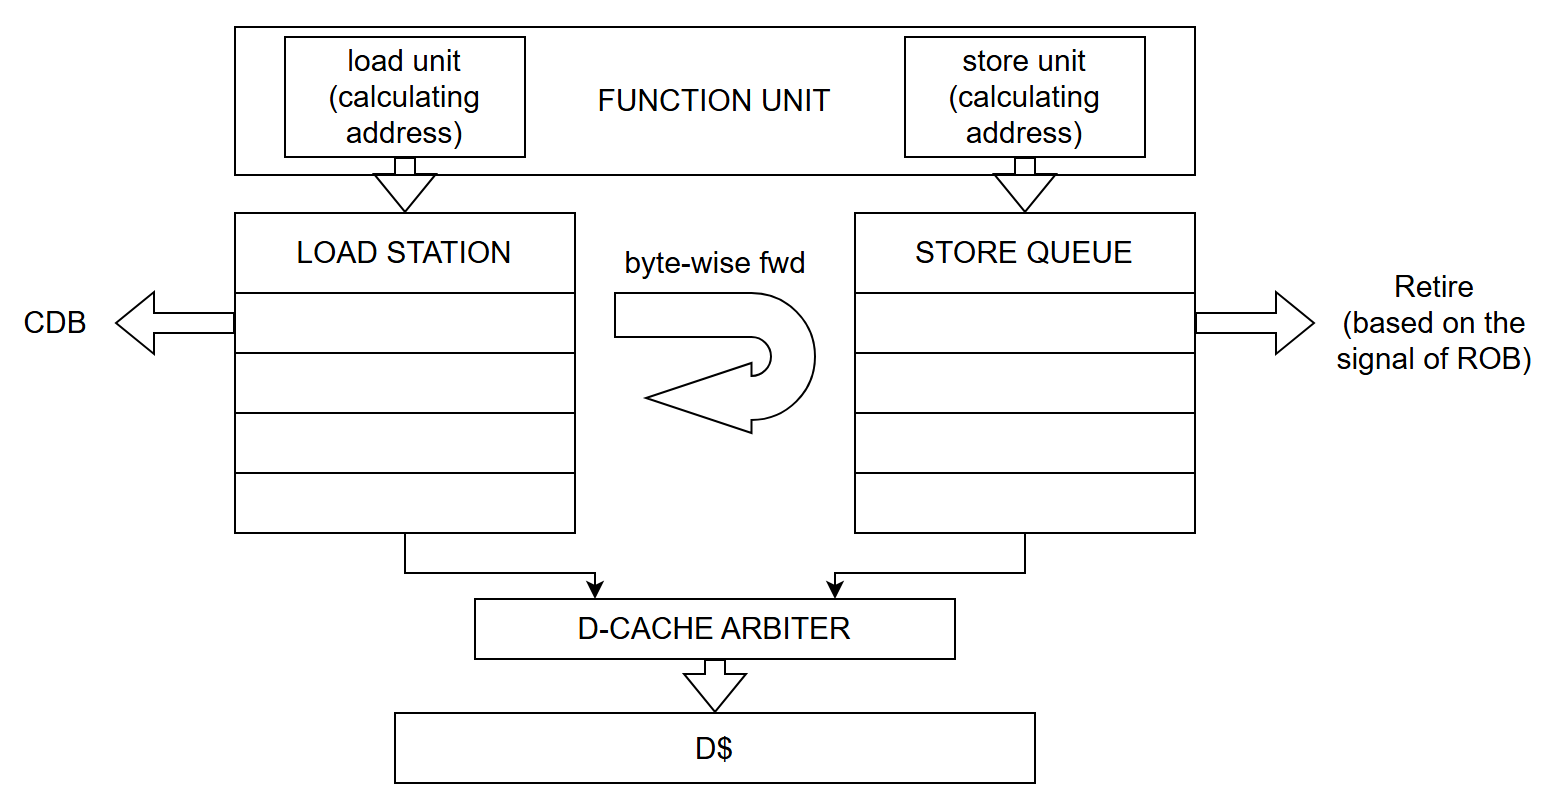
\includegraphics[width=0.3\textwidth]{figures/load_station.png}}
\caption{Load station and store queue layout.}
\label{fig:lsq}
\end{figure}

\subsubsection{Store Queue}

A store instruction will be allocated in SQ when dispatched. Then, after it is executed, the memory address and data will be stored in SQ. Then, it will send the store request to D-cache when it is retired in the ROB. If the D-cache is meeting a structural hazard, this cycle's attempt will fail, the retire will be stalled and it will repeat in the next cycle. 

\subsubsection{Load Station}

A load instruction receives an SQ (Store Queue) position indicating the tail, which helps track all prior store instructions when dispatched. The load is issued only when its source register is ready and all preceding stores have computed their addresses. This ensures at least one valid data source—either memory or the SQ. It leaves the station when gets the data and then goes to the complete stage. 

In the load station, it first gets forwarding data from the SQ before requesting data from the cache. The load station operates as an FSM. If a structural hazard with the D-cache prevents the request, it retries until successful. Upon receiving a cache response, a hit completes the operation, while a miss keeps the load waiting in the station.

To guarantee correct forwarding, we implement byte-wise forwarding. The logic treats the cache line as a unit: the SQ returns an entire cache line (shared with the load) along with a mask specifying forwarded bytes. When the load later receives cache data, it masks out these bytes to ensure correctness. 


\subsection{Branch Prediction}
Branch target addresses are predicted during the fetch stage, enabling the processor to fetch from the predicted target in the next cycle. We employ a GShare direction predictor, which leverages global history and program patterns to improve prediction accuracy. To predict target addresses, we employ a branch target buffer for general cases and a return address stack specifically for return statement predictions.

To balance complexity and latency, the predictor generates at most one branch prediction per cycle. This ensures efficient execution without incurring high prediction overhead.



\section{Result}
Our processor meets all baseline requirements and functions correctly under our various test approaches.

According to the iron law, the performance of our processor is mainly evaluated by $\frac{\#cycle}{\#inst}\times\frac{time}{cycle}$, i.e., CPI multiplied by clock period. We achieved \textbf{10ns clock period} in our final design, with a weighted average \textbf{CPI of 1.68}. Specific CPIs for each program are listed in Table I.

\begin{table}[htbp]
\centering
\label{ProgramCPI}
\caption{CPI for test programs (only .c program)}
\begin{tabular}{ll} 
\hline\hline
Program name      & CPI    \\ 
\hline
alexnet           & 1.530  \\
backtrack         & 2.285  \\
basic\_malloc     & 2.592  \\
bfs               & 1.910  \\
dft               & 1.545  \\
fc\_forward       & 1.611  \\
graph             & 2.274  \\
insertionsort     & 1.045  \\
matrix\_mult\_rec & 1.102  \\
mergesort         & 1.856  \\
omegalul          & 2.189  \\
outer\_product    & 1.002  \\
priority\_queue   & 2.646  \\
quicksort         & 1.679  \\
sort\_search      & 1.178  \\
\hline\hline
\end{tabular}
\end{table}


\section{Analysis}
\subsection{N-way Optimization}

We adjusted the CDB width to address a significant performance bottleneck observed when the width was set to 1. Specifically, with only one CDB available, the CDB stall rate reached approximately 45\%. This high stall rate caused functional units to be occupied longer and prevented completed instructions from writing their results back to the register file. As a result, dependent instructions could not be issued on time, stalling the pipeline and increasing overall CPI.
\begin{figure}[htbp]
  \centering
  \begin{minipage}[t]{0.24\textwidth}
    \centering
    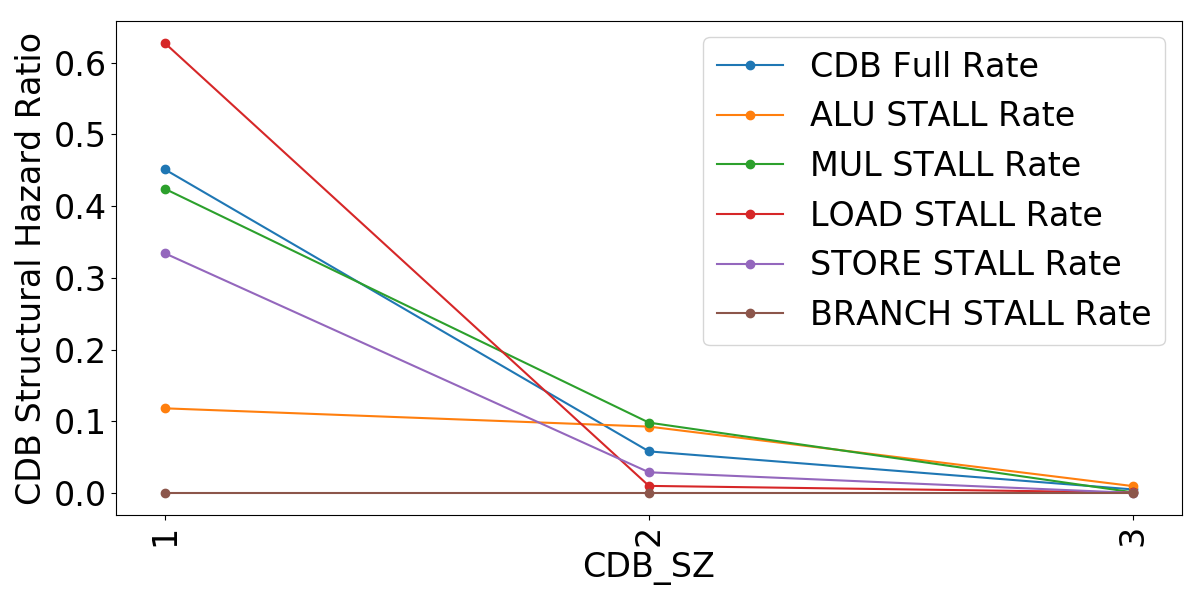
\includegraphics[width=\textwidth]{figures/Analysis/N-way/CDB_Stru.png}
    \caption{CDB Size vs. CDB Stall Rate}
    \label{fig:cdb_stall}
  \end{minipage}
  \hfill
  \begin{minipage}[t]{0.24\textwidth}
    \centering
    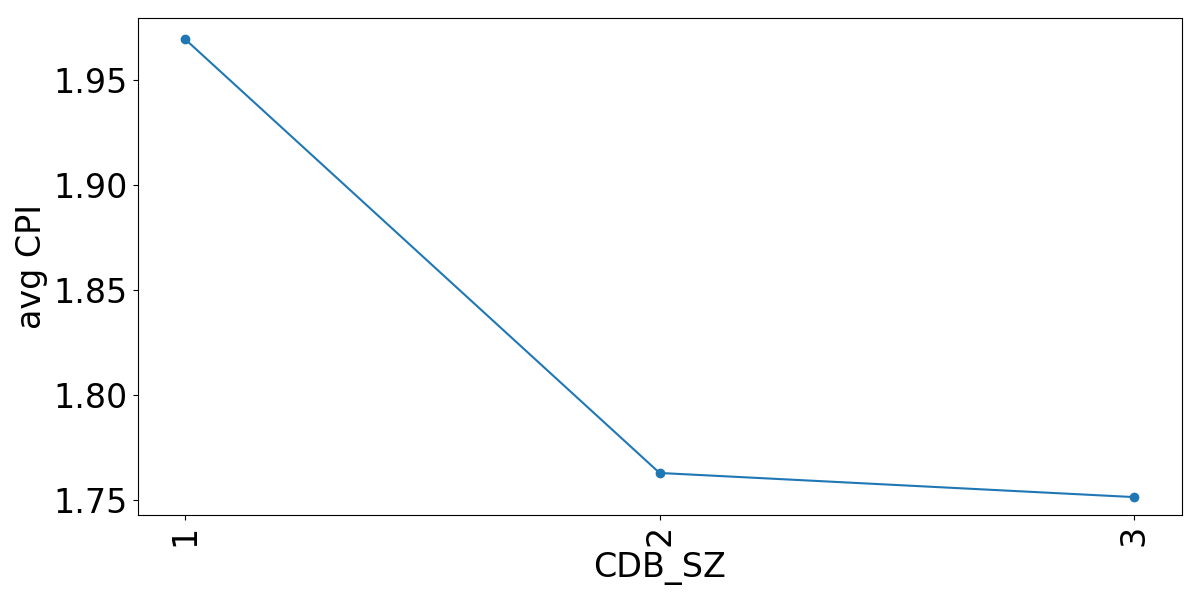
\includegraphics[width=\textwidth]{figures/Analysis/N-way/cpi_CDB.png}
    \caption{CDB Size vs. CPI}
    \label{fig:cdb_cpi}
  \end{minipage}
\end{figure}

The detailed result is shown in Figure~\ref{fig:cdb_stall}. We can see that the branch stall rate is always 0, and this is because we always prioritize branch instructions to resolve possible branch mispredictions earlier.

As shown in Figure~\ref{fig:cdb_stall}, each time the CDB width was increased by 1, the CDB stall rate dropped by approximately 8 times, and as shown in Figure~\ref{fig:cdb_cpi}, the CPI improved by roughly 10\%. These results demonstrate that increasing the CDB width effectively alleviates CDB bottlenecks, enabling faster instruction completion and reducing CPI.

\subsection{RS Size Optimization}
We initially configured the Reservation Station (RS) size to 8. However, this setup resulted in a high structural hazard rate of approximately 28\%, which prevented instructions from being dispatched. These stalls contributed to an increased CPI due to underutilization of functional units and pipeline inefficiency.
\begin{figure}[htbp]
  \centering
  \begin{minipage}[t]{0.24\textwidth}
    \centering
    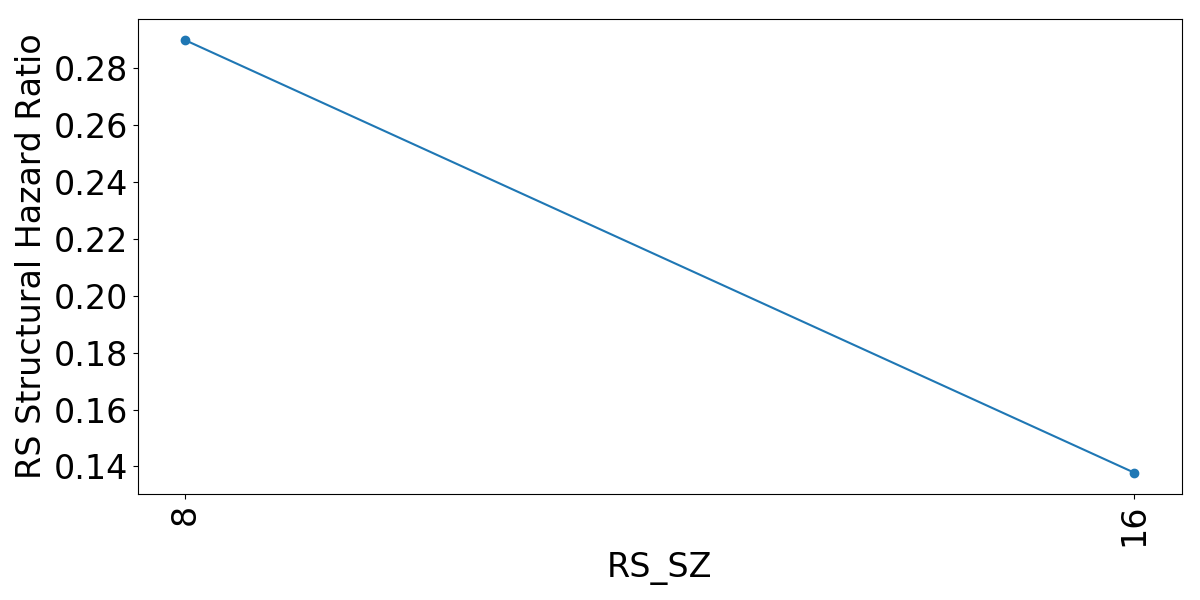
\includegraphics[width=\textwidth]{figures/Analysis/N-way/RS_Stru.png}
    \caption{RS Size vs. RS Full Rate}
    \label{fig:rs_stall}
  \end{minipage}
  \hfill
  \begin{minipage}[t]{0.24\textwidth}
    \centering
    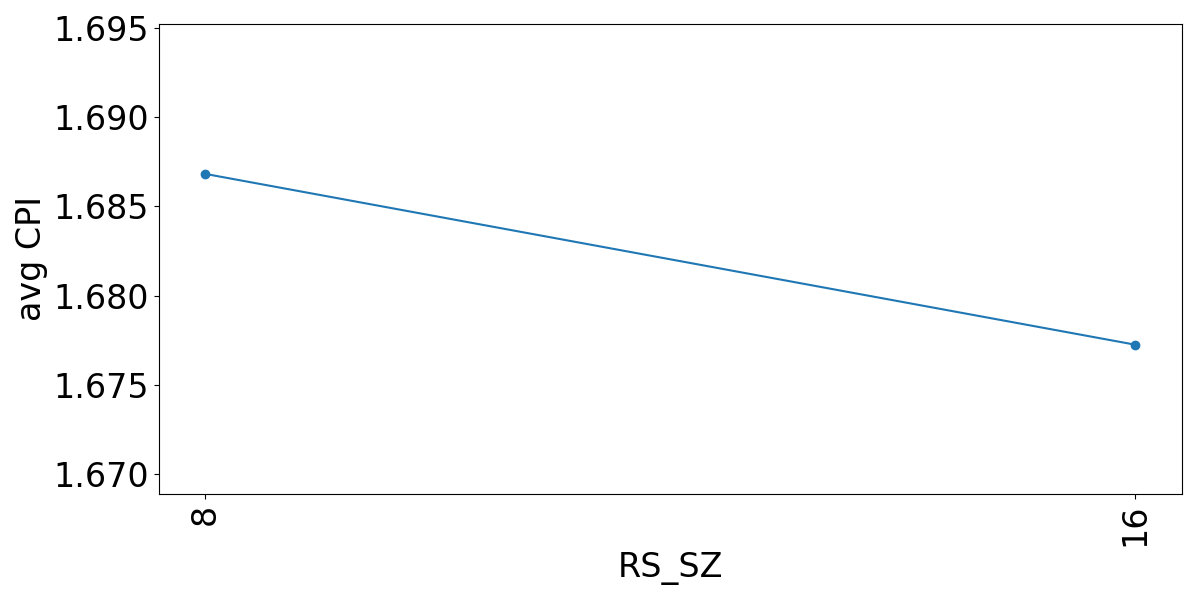
\includegraphics[width=\textwidth]{figures/Analysis/N-way/cpi_RS.png}
    \caption{RS Size vs. CPI}
    \label{fig:rs_cpi}
  \end{minipage}
\end{figure}
To alleviate this issue, we increased the RS size to 16. As shown in Figure~\ref{fig:rs_stall}, this optimization reduced the structural hazard rate by more than 50\% and as shown in Figure~\ref{fig:rs_cpi}, the reduction in CPI was about 0.5\%.
\subsection{ROB Size Optimization}
Initially, we set the Reorder Buffer (ROB) size to 24. However, this led to a noticeable performance issue: around 12\% of instructions encountered structural hazards during dispatch due to ROB entries being unavailable. As a result, pipeline stalls and the overall CPI is high.

To address this bottleneck, we experimented with resizing the ROB. Our results in Fig. \ref{fig:rob_stall} show that increasing the ROB size significantly reduced structural hazards—by approximately 50\%—which in turn lowered the CPI by 0.8\%, as shown in Fig. \ref{fig:rob_cpi}.
\begin{figure}[htbp]
  \centering
  \begin{minipage}[t]{0.24\textwidth}
    \centering
    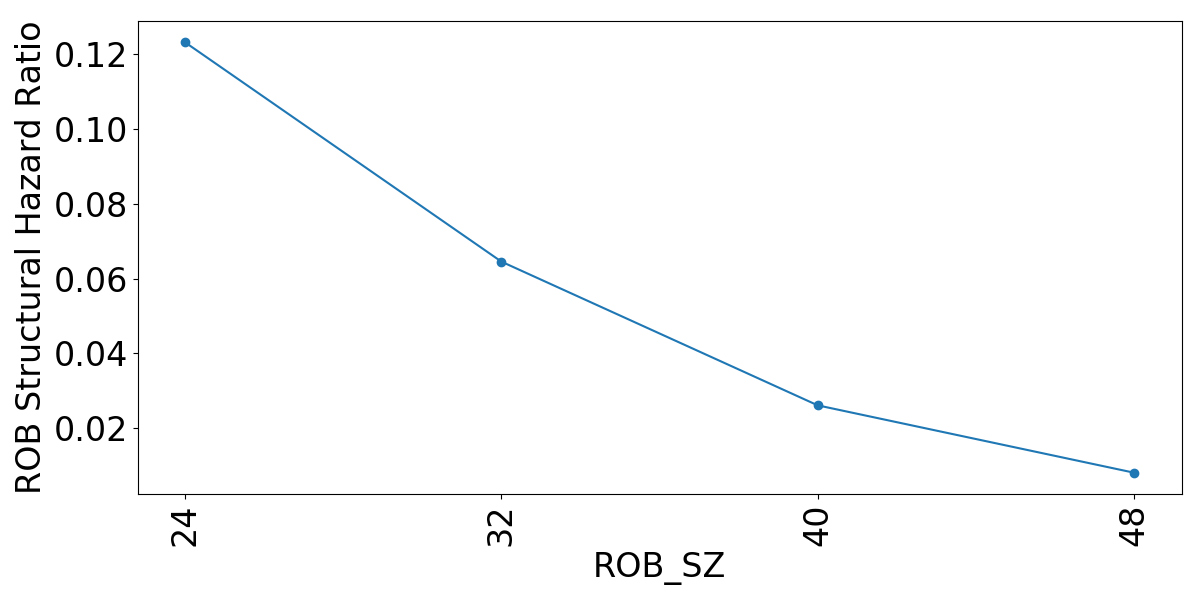
\includegraphics[width=\textwidth]{figures/Analysis/N-way/ROB_Stru.png}
    \caption{ROB Size vs. ROB Full Rate}
    \label{fig:rob_stall}
  \end{minipage}
  \hfill
  \begin{minipage}[t]{0.24\textwidth}
    \centering
    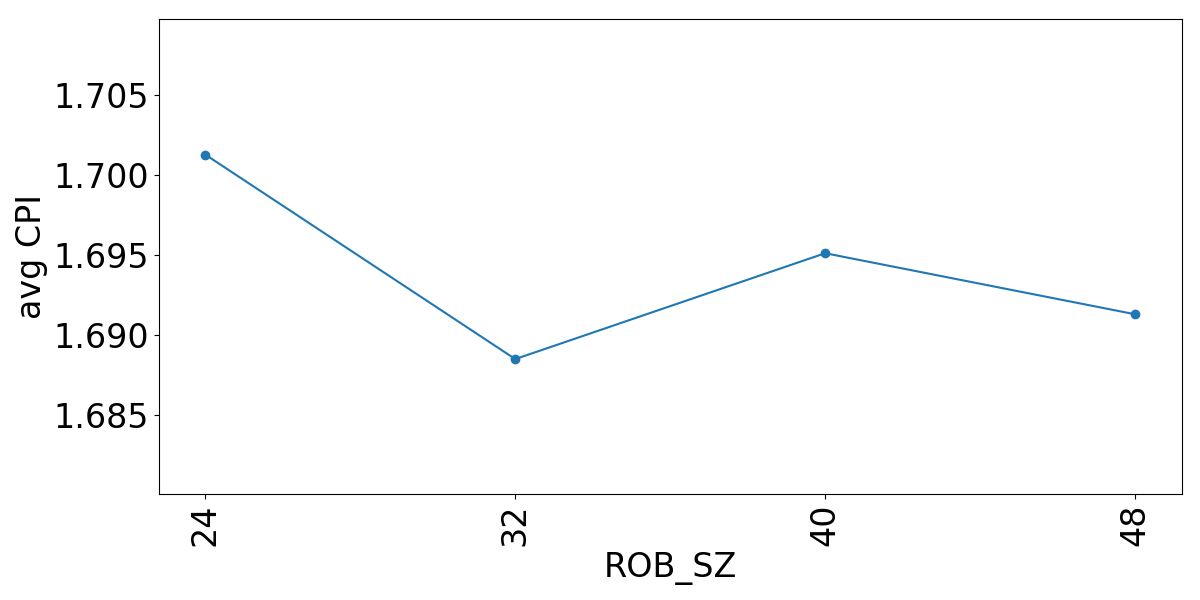
\includegraphics[width=\textwidth]{figures/Analysis/N-way/cpi_ROB.png}
    \caption{ROB Size vs. CPI}
    \label{fig:rob_cpi}
  \end{minipage}
\end{figure}
However, we also observed that beyond a certain point, further increasing the ROB size led to higher CPI. We hypothesize that this is because when too many instructions are waiting to be issued, backend resources become saturated. This causes newer instructions to occupy resources needed by older instructions, preventing them from completing and introducing stalls in a different part of the pipeline. Therefore, we finalized our ROB size to 32, and our ROB full rate is about 6\%.

\subsection{Prefetching}

With the transition to a 4-way instruction fetch, we observed a notable drop in instruction cache (i-cache) hit rates across several benchmark programs. To address this, we implemented a prefetching mechanism for the i-cache. Specifically, while serving pending fetch requests, we preemptively fetch subsequent instruction memory blocks into a stream buffer. This technique helps maintain a steady flow of useful requests to memory, thereby better utilizing available memory bandwidth.

The size of the stream buffer plays a critical role in overall CPI, as illustrated in Figure~\ref{PrefetchBufferSize}. Increasing the buffer size from 2 to 4 entries resulted in up to a 50\% reduction in CPI for certain workloads.

\begin{figure}[htbp]
\centerline{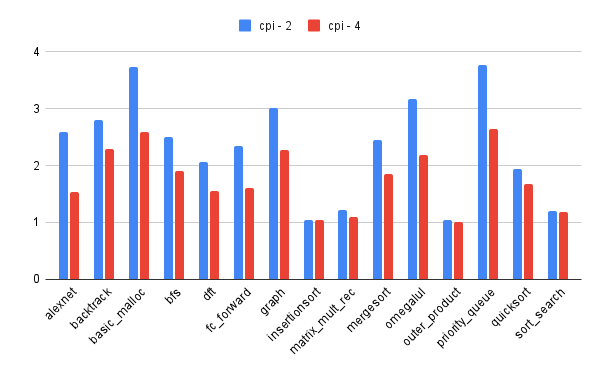
\includegraphics[width=0.8\columnwidth]{Analysis/PrefetchBufferSize}}
\caption{Impact of Prefetch Buffer Size on CPI. Blue bars correspond to a size of 2; red line indicates results for size 4.}
\label{PrefetchBufferSize}
\end{figure}

From the hit rate data in Figure~\ref{ICacheHitRate}, it is evident that the stream buffer size is a significant bottleneck in the fetch stage. Given constraints on buffer capacity, one potential optimization is to more aggressively promote data from the stream buffer into the i-cache, improving the likelihood of hits and reducing fetch stalls.

\begin{figure}[htbp]
\centerline{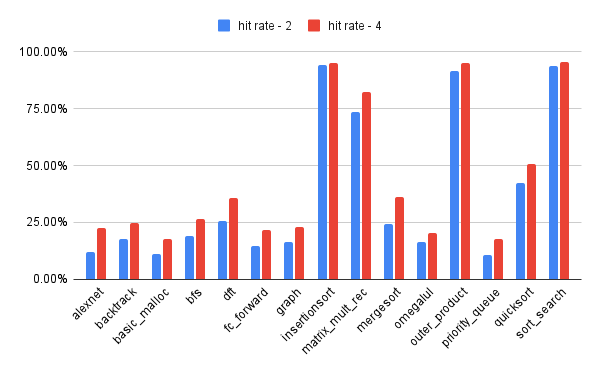
\includegraphics[width=0.7\columnwidth]{Analysis/ICacheHitRate}}
\caption{Instruction Cache Hit Rate vs. Stream Buffer Size}
\label{ICacheHitRate}
\end{figure}

\subsection{Banked Instruction Cache}

To support 4-way instruction fetch, we often need to access two instruction memory blocks concurrently. However, our original i-cache design featured only a single read port, making such parallel access infeasible. To resolve this, we modified the i-cache to include two independent banks, enabling simultaneous dual-block access. This architectural change led to an average CPI reduction of approximately 1\%.

\subsection{Issuing with Age-Based Logic}

In the baseline design, the issue logic selects instructions for execution in a pseudo-random fashion. Ideally, the processor should issue instructions whose execution will unlock the greatest number of dependent instructions. While tracking all dependencies precisely would be prohibitively complex, a useful heuristic is to prioritize older instructions, as they are more likely to have dependent operations waiting in the pipeline.

This strategy becomes particularly relevant when the number of ready reservation station entries exceeds the available functional unit or CDB capacity. To quantify this, we define the issue rate as:

$$
\frac{\text{\#entries\_issued}}{\text{\#entries\_ready}}
$$

Figure~\ref{IssueRate} shows the issue rate across various benchmarks.

\begin{figure}[htbp]
\centerline{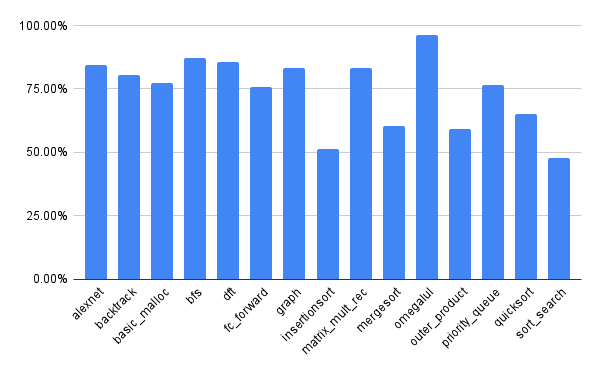
\includegraphics[width=0.6\columnwidth]{Analysis/IssueRate}}
\caption{Issue Rate Across Benchmarks}
\label{IssueRate}
\end{figure}

In several programs, the issue rate hovers around 50\%, suggesting that age-based issuing has the potential to improve performance by making better use of available execution resources.

The performance impact of this heuristic is shown in Figure~\ref{AgeLogic}.

\begin{figure}[htbp]
\centerline{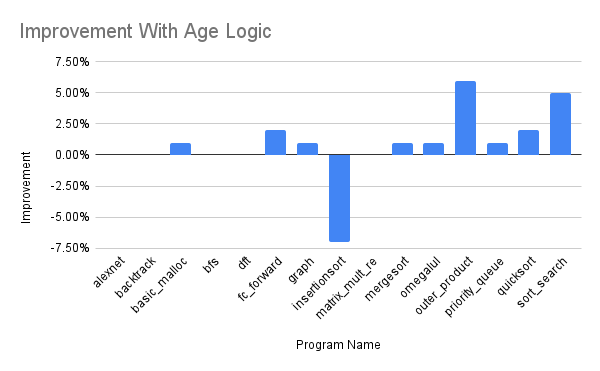
\includegraphics[width=0.7\columnwidth]{Design/AgeLogic}}
\caption{Performance Impact of Age-Based Issuing}
\label{AgeLogic}
\end{figure}

On average, we observed a modest 1.5\% improvement in performance. However, some programs experienced a noticeable performance degradation. This suggests that in certain scenarios, issuing younger instructions can unlock more parallelism than strictly following program order. Furthermore, the added complexity of age-based logic introduced non-trivial latency to the issue stage. Based on these trade-offs, we ultimately chose to revert to the simpler, baseline issue logic.

\subsection{Return Address Stack}

Return instructions exhibit a unique behavior compared to other branch instructions. Unlike branches with fixed offsets, return instructions do not have a predetermined target, which can make them difficult for the Branch Target Buffer (BTB) to predict. However, return instructions always target the location from which the function was originally called. In theory, this makes it possible to predict return instructions with high precision.

In practice, though, programs with deep call stacks can cause structural hazards in the Return Address Stack (RAS). One potential solution is to stall the fetch stage until the structural hazard is resolved. However, we aim to maintain the fundamental behavior of the processor without altering the branch prediction unit. If our RAS implementation is flawed—for instance, if we mistakenly treat ordinary jump instructions as return instructions—the processor may no longer work correctly.

To mitigate the structural hazard, we chose to increase the size of the RAS. Our benchmarks show that increasing the RAS size from 4 to 8 entries reduces the frequency of structural hazards from 80\% to 20\%, with a corresponding 1.5\% increase in CPI. Further increasing the RAS size beyond this point provides diminishing gains, as shown in Figure~\ref{RASSize}.

\begin{figure}[htbp]
\centerline{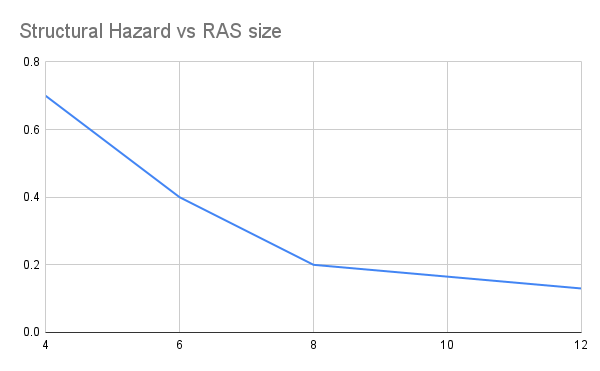
\includegraphics[width=0.6\columnwidth]{Analysis/RASSize}}
\caption{Structural Hazard Rate}
\label{RASSize}
\end{figure}


\subsection{Dcache Optimization}
\label{sec:dcache-opti}

Our goal is to reduce CPI by alleviating conflict misses in the L1 D‑cache.  Table~\ref{tab:cache-comparison} shows that a \emph{direct‑mapped} cache suffers from relatively low hit rates (mid‑80\%–low‑90\%), which drives up CPI.

\subsubsection{From Direct‑Mapped to 2‑Way}
Moving to a 2‑way set‑associative cache yields the largest benefits:
\begin{itemize}
  \item \textbf{Hit‑Rate Lift:} For most benchmarks, hit rate increases by 3–16\% points.
  \item \textbf{CPI Reduction:} Corresponding CPI drops by 5–23\%; for example, \texttt{matrix\_mult\_rec} sees its CPI fall from 1.103 to 0.852.
\end{itemize}
Figure~X plots CPI vs.\ cache type and clearly shows a sharp “step” improvement when going from direct‑mapped to 2‑way.

\subsubsection{From 2‑Way to 4‑Way: Diminishing Returns}
Further increasing associativity to 4‑way yields only marginal gains:
\begin{itemize}
  \item \textbf{Hit‑Rate Change:} Most programs' hit rate gain at most 1–2\%, and a few (e.g. \texttt{backtrack}) actually dip slightly.
  \item \textbf{CPI Impact:} The CPI curves flatten out—conflict misses were already largely eliminated by 2‑way.
  \item \textbf{Hardware Cost and Timing:}
    \begin{itemize}
      \item \emph{Synthesis Violations:} After synthesis, the 4‑way design exhibits timing violations on the path from the function unit to the D‑cache of \SI{5.50}{\nano\second}, and on the path from the memory interface to the D‑cache of \SI{0.36}{\nano\second}.
      \item These violations complicate timing closure and may require lowering clock frequency or adding pipeline stages.
    \end{itemize}
\end{itemize}

\noindent
Therefore, the 2‑way set‑associative design represents the best trade‑off between performance (hit rate \& CPI) and implementation complexity.
\begin{table}[ht]
\centering
\caption{CPI and Hit Rate Comparison}
\label{tab:cache-comparison}
\begin{tabular}{l
                rrr  % CPI: DM, 2‑Way, 4‑Way
                rrr} % Hit Rate: DM, 2‑Way, 4‑Way
\toprule
Program & \multicolumn{3}{c}{CPI} & \multicolumn{3}{c}{Hit Rate (\%)} \\
\cmidrule(lr){2-4} \cmidrule(lr){5-7}
        & DM      & 2‑Way   & 4‑Way   & DM     & 2‑Way  & 4‑Way  \\
\midrule
alexnet             & 1.530 & 1.500 & 1.498 & 93.48 & 97.16 & 97.24 \\
backtrack           & 2.286 & 2.145 & 2.156 & 89.89 & 94.22 & 93.59 \\
basic\_malloc        & 2.592 & 2.609 & 2.600 & 92.50 & 94.55 & 94.82 \\
bfs                 & 1.910 & 1.892 & 1.889 & 93.33 & 94.94 & 95.12 \\
dft                 & 1.546 & 1.549 & 1.545 & 96.70 & 96.24 & 97.62 \\
fc\_forward         & 1.611 & 1.544 & 1.544 & 83.72 & 89.64 & 89.24 \\
graph               & 2.274 & 2.254 & 2.242 & 93.99 & 95.36 & 95.76 \\
insertionsort       & 1.047 & 1.045 & 1.045 & 97.09 & 96.93 & 96.45 \\
matrix\_mult\_rec   & 1.103 & 0.852 & 1.093 & 41.46 & 58.25 & 42.20 \\
mergesort           & 1.856 & 1.805 & 1.795 & 94.15 & 96.05 & 96.52 \\
omegalul            & 2.189 & 2.189 & 2.189 & 64.71 & 64.71 & 64.71 \\
outer\_product      & 1.004 & 0.963 & 0.934 & 88.87 & 93.47 & 95.26 \\
priority\_queue     & 2.647 & 2.620 & 2.617 & 90.44 & 94.03 & 93.74 \\
quicksort           & 1.680 & 1.608 & 1.601 & 94.27 & 96.25 & 96.56 \\
sort\_search        & 1.179 & 1.154 & 1.159 & 97.42 & 98.01 & 97.76 \\
\bottomrule
\end{tabular}
\end{table}

\subsection{Load Station Size Optimization}
Initially, we make the load station size 4. Then by statistics, we've found that there are about \%2.7 of the time the load station is full. There might be potential for more load to be waiting in the load station at the same time, which can make memory request happens earlier and then improve the CPI. Therefore, we initiate a load station size optimization. We've attempted to change the size of the load station to fully leverage its potential in improving the performance. Here we changed the size from 1 to 5. And we are recording the normalized performance, which is calculated by \ref{eq:load_size}. We are all comparing with the situation of size 4. 

\begin{equation}
\text{Normalized Performance}_i=\frac{\text{CPI}_{\text{N=4}}}{\text{CPI}_{\text{N=i}}} 
\label{eq:load_size}
\end{equation}


From Fig. \ref{fig:load_size} we can see that the performance improved dramatically whenthe  size changes from 1 to 3. However, there's almost no improvement when the size changes from 4 to 5. Since load station is not on the critical path, there's no need to make it smaller. Finally, we just keep it at the size of 4. We have already exploited its potential. 


\begin{figure}[htbp]
\centerline{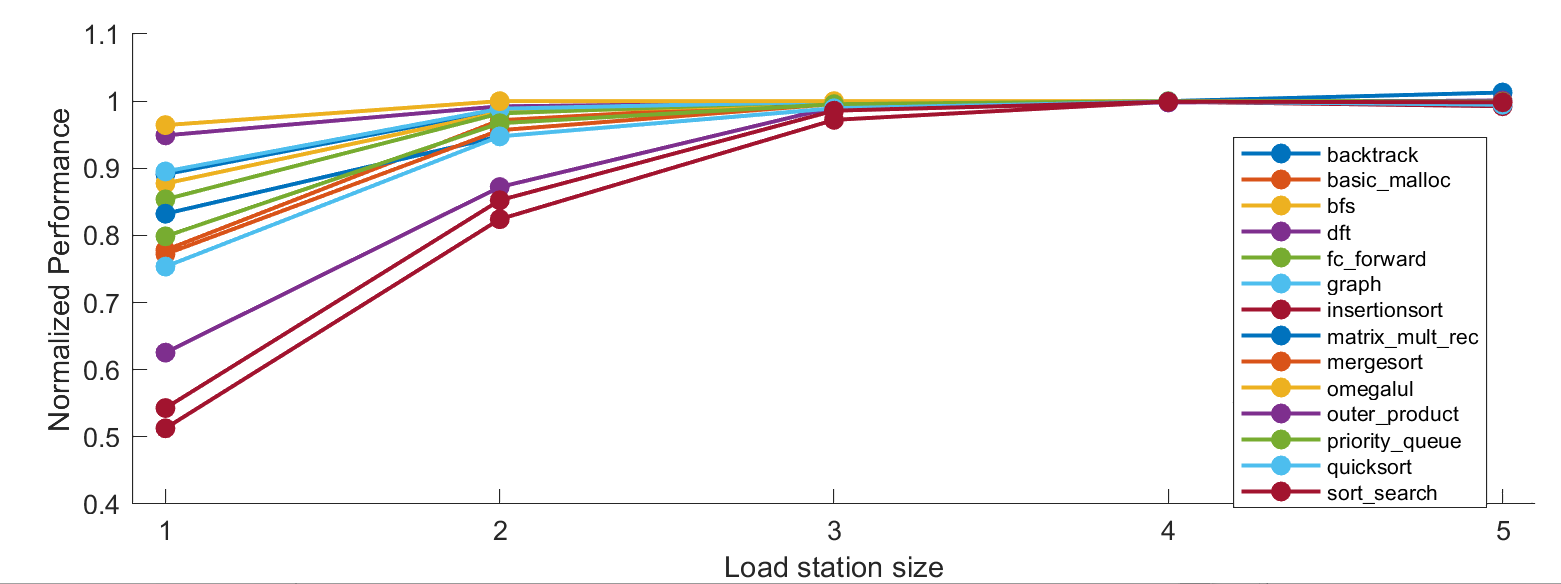
\includegraphics[width=0.5\textwidth]{figures/Analysis/load_size.png}}
\caption{Performance vs load station size.}
\label{fig:load_size}
\end{figure}

\subsection{Optimization attempts of branch predictor}
We finally settled on Gshare because it turned out to be the most robust in practice. Along the way, we also built TAGE-like, perceptron, 1-layer CNN, and N-layer CNN branch predictors. We compared their overall performance, using Gshare with a BHR length of 8 as the baseline. The summary tables are shown below. The comparative bar chart is included in the appendix.
\begin{table}[ht]
  \scriptsize
  \setlength{\tabcolsep}{2pt}           
  \caption{CPI–program relation}
  \label{tab:branch-cpi}
  \begin{tabular*}{\columnwidth}{@{\extracolsep{\fill}}lccccc}
    \toprule
    Program & Gshare & TAGE & Perceptron & 1-layer CNN & N-layer CNN \\
    \midrule
    alexnet           & 1.530 & 1.703 & 1.482 & 1.872 & 1.881 \\
    backtrack         & 2.285 & 2.422 & 2.219 & 2.389 & 2.486 \\
    basic\_malloc     & 2.592 & 2.722 & 2.620 & 2.622 & 2.734 \\
    bfs               & 1.910 & 1.915 & 1.797 & 2.045 & 1.872 \\
    dft               & 1.545 & 1.634 & 1.507 & 1.783 & 1.618 \\
    fc\_forward       & 1.611 & 1.624 & 1.528 & 1.579 & 1.531 \\
    graph             & 2.274 & 2.324 & 2.223 & 2.298 & 2.377 \\
    insertionsort     & 1.045 & 1.233 & 1.030 & 2.711 & 1.012 \\
    matrix\_mult\_rec & 1.102 & 1.114 & 1.107 & 2.303 & 1.121 \\
    mergesort         & 1.856 & 1.952 & 1.858 & 1.979 & 2.087 \\
    omegalul          & 2.189 & 2.189 & 2.175 & 2.189 & 2.189 \\
    outer\_product    & 1.002 & 1.012 & 0.968 & 1.320 & 1.000 \\
    priority\_queue   & 2.646 & 2.773 & 2.760 & 2.665 & 2.793 \\
    quicksort         & 1.679 & 1.814 & 1.672 & 1.963 & 1.697 \\
    sort\_search      & 1.178 & 1.298 & 1.144 & 2.034 & 1.167 \\
    \bottomrule
  \end{tabular*}
\end{table}

\begin{table}[ht]
  \scriptsize
  \setlength{\tabcolsep}{2pt}
  \caption{Hit-rate(\%)–program relation}
  \label{tab:branch-hit}
  \begin{tabular*}{\columnwidth}{@{\extracolsep{\fill}}lccccc}
    \toprule
    Program & Gshare & TAGE & Perceptron & 1-layer CNN & N-layer CNN \\
    \midrule
    alexnet           & 86.94 & 75.52 & 91.56 & 58.69 & 48.91 \\
    backtrack         & 68.02 & 67.16 & 78.04 & 61.71 & 65.15 \\
    basic\_malloc     & 56.03 & 63.85 & 63.64 & 57.85 & 59.32 \\
    bfs               & 58.95 & 70.65 & 75.45 & 53.48 & 71.62 \\
    dft               & 82.63 & 71.14 & 86.57 & 38.61 & 71.68 \\
    fc\_forward       & 20.00 & 45.45 & 63.64 & 50.00 & 63.64 \\
    graph             & 60.61 & 62.82 & 68.85 & 54.03 & 60.87 \\
    insertionsort     & 94.88 & 87.15 & 95.96 & 51.15 & 96.05 \\
    matrix\_mult\_rec & 97.91 & 96.56 & 98.28 & 51.79 & 97.42 \\
    mergesort         & 72.64 & 69.01 & 78.27 & 65.46 & 69.65 \\
    omegalul          &  0.00 &  0.00 &  0.00 &  0.00 &  0.00 \\
    outer\_product    & 93.88 & 89.95 & 98.58 & 71.30 & 94.36 \\
    priority\_queue   & 54.27 & 62.29 & 58.75 & 59.65 & 56.52 \\
    quicksort         & 73.99 & 74.61 & 79.15 & 43.49 & 81.58 \\
    sort\_search      & 89.53 & 83.32 & 91.69 & 56.43 & 90.87 \\
    \bottomrule
  \end{tabular*}
\end{table}

\subsubsection{Gshare predictor}

Gshare forms its PHT index by XOR’ing the fetch‐stage PC’s low bits with the global BHR.  That index drives a two-bit counter to make a speculative prediction during fetch; once the real outcome is known, the predictor restores its snapshot and updates both the counter and the BHR accordingly.

\paragraph{Fetch phase.}  Let $h=\texttt{BHR\_SIZE}$.  Compute the fetch index and prediction as
\begin{IEEEeqnarray}{rCl}
  \mathrm{Idx}_{\mathrm{fetch}}
    &=& \texttt{fetch\_pc}[h-1:0]\;\oplus\;\mathrm{BHR}_t,
  \label{eq:idx-fetch}\\
  \hat{T}
    &=& \begin{cases}
          1, & C_t[\mathrm{Idx}_{\mathrm{fetch}}]\ge 2,\\
          0, & C_t[\mathrm{Idx}_{\mathrm{fetch}}]\le 1.
        \end{cases}
  \label{eq:pred-fetch}
\end{IEEEeqnarray}
Speculatively update both BHR and counter:
\begin{IEEEeqnarray}{rCl}
  \mathrm{BHR}_{t+1}
    &=& \bigl\{\mathrm{BHR}_t[h-2:0],\,\hat{T}\bigr\},
  \label{eq:bhr-update-fetch}\\
  C_{t+1}[\mathrm{Idx}_{\mathrm{fetch}}]
    &=& \begin{cases}
          \min\bigl(C_t[\mathrm{Idx}_{\mathrm{fetch}}]+1,3\bigr), & \hat{T}=1,\\
          \max\bigl(C_t[\mathrm{Idx}_{\mathrm{fetch}}]-1,0\bigr), & \hat{T}=0,\\
          
        \end{cases}
  \label{eq:pht-update-fetch}
\end{IEEEeqnarray}
Parallel snapshots of BHR and PHT are stored in indexed “copies” at each fetch so that mis‐speculation may be rolled back.

\subsubsection{TAGE-like predictor}

Inspired by Seznec et al.’s work, this module extends the classical gshare predictor by attaching a tag and a “useful” bit to each two‐bit saturating counter entry and by supporting periodic aging (decay) of the useful bits.  The prediction state is maintained in a global Branch History Register (BHR) of width $h$, and in a Pattern History Table (PHT) of size $2^h$ whose entries are
\[
\mathtt{pht}[i]
  = \bigl(
      \underbrace{\mathrm{ctr}_i}_{\text{2‐bit counter}},\;
      \underbrace{\mathrm{tag}_i}_{\ell\text{-bit tag}},\;
      \mathrm{valid}_i,\;
      \mathrm{useful}_i
    \bigr)\,.
\]
Speculative updates are stored in parallel “copies” indexed by the fetch‐stage buffer index; on resolution a saved copy is restored before applying the true outcome update.

\paragraph{Fetch and speculative update.}  
Given the fetch‐stage PC and BHR,
{\small
\begin{IEEEeqnarray}{rCl}
  \mathrm{Idx}
    &=
    &\mathrm{PC}[\,h-1:0\,]\;\oplus\;\mathrm{BHR}_t,
  \label{eq:dirpred-idx}\\
  \mathrm{tag}   
    &=
    &\bigl(\mathrm{PC}[\,h-1:0\,]\!\gg3\bigr)
      \;\oplus\;\mathrm{BHR}_t\;\oplus\;(\mathrm{BHR}_t\ll1)
  \label{eq:dirpred-tag}
\end{IEEEeqnarray}
}
An entry matches if \(\mathrm{valid}_{\mathrm{Idx}}=1\) and \(\mathrm{tag}_{\mathrm{Idx}}=\mathrm{tag}\).  If no match or entry not useful, a new entry is allocated:
\[
\begin{cases}
  \mathrm{ctr}_{\mathrm{Idx}}\leftarrow\mathtt{01},\\
  \mathrm{tag}_{\mathrm{Idx}}\leftarrow\mathrm{tag},\\
  \mathrm{valid}_{\mathrm{Idx}}\leftarrow1,\quad \mathrm{useful}_{\mathrm{Idx}}\leftarrow0.
\end{cases}
\]
Otherwise, the prediction is
\[
\hat{T}
=\bigl(\mathrm{ctr}_{\mathrm{Idx}}\ge2\bigr)\,,
\mathrm{useful}_{\mathrm{Idx}}\leftarrow1
\]
and the counter and useful bit update is similar to Gshare.

\paragraph{Resolution and recovery.}  
Upon resolution of a mis‐prediction at time $t+\delta$, the branch resolution logic is similar to Gshare predictor.
A free-running \(\mathtt{decay\_counter}\) resets all \(\mathrm{useful}_i\leftarrow0\) when it overflows, enabling periodic aging of table entries.

\paragraph{High-level selector}  

The TAGE-like predictor instantiates three \texttt{extended gshare} predictors with history lengths $h\in\{2,4,8\}$. We select among all predictions that match the tag and are useful, and prioritize the one with the longest history.

\subsubsection{Perceptron predictor}

Inspired by Jimemez et al.’s work, the perceptron predictor maintains a table of $N=2^m$ entries, each entry consisting of a bias $w_0$ and $h$ history weights $w_1,\dots,w_h$.  Let the global history bits $H_i\in\{+1,-1\}$ for $i=0,\dots,h-1$ be mapped from taken/not‐taken.  A hashed index selects one perceptron:
\[
\mathrm{Idx} = \mathrm{PC}[\,m-1:0\,]\;\oplus\;\mathrm{BHR}_t\,. 
\]
The \emph{dot–product} is
\begin{IEEEeqnarray}{rCl}
y &=& w_0 \;+\;\sum_{i=1}^{h} w_i\,H_{i-1},
\end{IEEEeqnarray}
and the prediction is
\[
\hat T = (y \ge 0)\,. 
\]
We update only if $\hat T \neq T$ or $|y|<\Theta$, where $\Theta$ is the training threshold(to guarantee high confidence).  The weight update rules are
\begin{IEEEeqnarray}{rCl}
w_i &\leftarrow& \mathrm{sat}\bigl(w_i + T\,H_{i-1}\bigr),\quad i=1,\dots,h,
  \label{eq:perc-update-weights}\\
w_0 &\leftarrow& \mathrm{sat}\bigl(w_0 + T\bigr),
  \label{eq:perc-update-bias}
\end{IEEEeqnarray}
where $W_{\max}=2^{b-1}-1$ for a $b$-bit signed weight and saturation function ensures won't exceed the limit.  

This design yields a simple linear predictor whose accuracy increases with history length while remaining implementable in hardware via integer arithmetic and small tables.

\subsubsection{One‐Layer CNN Predictor}

Inspired by Mao et al.’s work, the one‐layer CNN predictor applies a bank of $J$ 1D convolutional filters of width $K$ to the global history bits, followed by a single fully‐connected (FC) layer and a sign‐threshold decision.  Speculative state is saved in per‐fetch copies and recovered on mis‐prediction, analogous to gshare.

\paragraph{Convolution \& activation.}  Let $H_i\in\{+1,-1\}$ be the mapped history bits and $w_{j,k}$ the $k$th weight of filter $j$ ($k=0,\dots,K-1$).  The pre‐activation convolution output is
\begin{IEEEeqnarray}{rCl}
z_j
  &=& \sum_{i=0}^{h-K} \sum_{k=0}^{K-1} w_{j,k}\,H_{\,i+k}\,,
  \label{eq:cnn‐conv}\\
c_j
  &=& \max\bigl(z_j,\,0\bigr)\quad(\text{ReLU})\,.
  \label{eq:cnn‐relu}
\end{IEEEeqnarray}

\paragraph{Fully‐connected \& decision.}  With bias $b$ and FC weights $\alpha_j$, compute
\begin{IEEEeqnarray}{rCl}
y
  &=& b \;+\;\sum_{j=0}^{J-1} \alpha_j\,c_j,
  \label{eq:cnn‐fc}\\
\hat T
  &=& (y > 0)\,. 
  \label{eq:cnn‐pred}
\end{IEEEeqnarray}

\paragraph{History update and resolution}  After committing $\hat T$, the global history register is shifted in:
\[
\mathrm{BHR}_{t+1}
  \;=\;\bigl\{\mathrm{BHR}_t[h-2:0],\,\hat T\bigr\}\,.
\]
Its resolution is similar to what's in Gshare.
Together, these steps implement a hardware‐friendly CNN branch predictor: a small number of filter operations, ReLU activation, and a simple linear decision, with speculative state management mirroring the gshare mechanism.  

\subsubsection{Multi‐Layer CNN Predictor}

Inspired by Mao et al.’s work, the multi‐layer CNN predictor extends the one‐layer design by cascading $L$ convolution–binarization stages to extract progressively higher‐order history patterns, followed by a final fully‐connected decision.  Speculative state (the global BHR and its per‐fetch copies) is managed exactly as in the one‐layer predictor, ensuring simple recovery on mis‐prediction.

\paragraph{1. Branch‐History Recovery}  
The recovery of BHR in an n-layer CNN predictor is the same as 1-layer CNN.

\paragraph{2. Convolution \& Binarization Chain}  
Define the binary‐mapped history bits for layer $0$ as
\[
c^{(0)}_{p} = 
\begin{cases}
+1, & \mathrm{BHR}_{\mathrm{rec}}[p]=1,\\
-1, & \mathrm{BHR}_{\mathrm{rec}}[p]=0,
\end{cases}
\quad p=0,\dots,h-1.
\]
For each layer $\ell=1,\dots,L$ with $K_{\ell}$‐wide kernels and $F_{\ell}$ filters, the convolution and activation are
\begin{IEEEeqnarray}{rCl}
z^{(\ell)}_{j}
  &=& \sum_{p=0}^{F_{\ell-1}-K_{\ell}}
        \sum_{k=0}^{K_{\ell}-1}
        w^{(\ell)}_{j,k}\;c^{(\ell-1)}_{\,p+k},
  \label{eq:detailed-mlcnn-conv}\\
c^{(\ell)}_{j}
  &=& \bigl(z^{(\ell)}_{j}>0\bigr),
  \quad j=0,\dots,F_{\ell}-1,
  \label{eq:detailed-mlcnn-binarize}
\end{IEEEeqnarray}
where $F_{0}=h$ and $c^{(\ell)}_{j}\in\{0,1\}$ is the binary ReLU of the convolution result.

\paragraph{3. Fully‐Connected Scoring \& Prediction}  
The outputs of the final convolution layer $c^{(L)}_{j}$ feed a simple linear classifier with bias $b$ and weights $\alpha_{j}$:
\begin{IEEEeqnarray}{rCl}
y
  &=& b \;+\;\sum_{j=0}^{F_{L}-1} \alpha_{j}\,c^{(L)}_{j},
  \label{eq:detailed-mlcnn-fc}\\
\hat{T}
  &=& (y>0)\,,
  \label{eq:detailed-mlcnn-pred}
\end{IEEEeqnarray}
producing the branch‐taken prediction $\hat T\in\{0,1\}$.

\paragraph{4. History Update \& Speculative Snapshot}  
After prediction, the next global history is
\[
\mathrm{BHR}_{t+1}
=\{\mathrm{BHR}_{\mathrm{rec}}[h-2:0],\,\hat T\}.
\]
This new history is written back to the architectural BHR register. One of the advantages of n-layer-CNN is that it doesn't have any complicated recovery logic. This structure is promising to be used on pipelines with multi-stage branch prediction. 

\vspace{6pt}
By stacking small, binary‐activated convolutional filters and a lightweight linear classifier, this predictor captures non‐local history correlations with minimal control overhead, while inheriting the robust recovery mechanism of GShare.  

\subsection{Optimization Attempts of Branch Target Buffer}

In this subsection, we present our optimization strategies and experimental results for improving the performance of the Branch Target Buffer (BTB). We evaluated several aspects including BTB size, associativity, eviction policies, warm-up strategies, and integration with branch history. Our goal was to reduce the BTB miss rate and, consequently, improve the overall CPI (Cycles Per Instruction) of the program. The following tests are all done on short programs.

\subsubsection{Miss Rate Calculation}

The BTB miss rate is defined as the ratio of missed conditional and taken branches to the total number of conditional branches. Formally, we compute:

\[
\text{Miss Rate} = \frac{\#(\text{missed} \land \text{taken} \land \text{conditional})}{\#(\text{conditional branches})}
\]

This metric directly influences the control hazard penalty, making it a crucial indicator of BTB effectiveness.

\subsubsection{Direct-Mapped BTB Performance with Varying Sizes}

We first explored how increasing the size of a direct-mapped BTB affects performance. The miss rate decreases significantly as we increase the number of entries, but the improvement plateaus after a certain threshold due to diminishing returns. Below is a plot (omitted in this snippet) that shows this trend.

\begin{center}
\begin{tabular}{|c|c|}
\hline
\textbf{BTB Size (entries)} & \textbf{Miss Rate} \\
\hline
16 & 0.2529 \\
32 & 0.1876 \\
64 & 0.0867 \\
128 & 0.0820 \\
\hline
\end{tabular}
\end{center}

We observed a large performance gain up to 32 entries. Beyond that, the gain becomes marginal, suggesting 32 as a good trade-off point between performance and storage.
\begin{figure}[htbp]
    \centering
    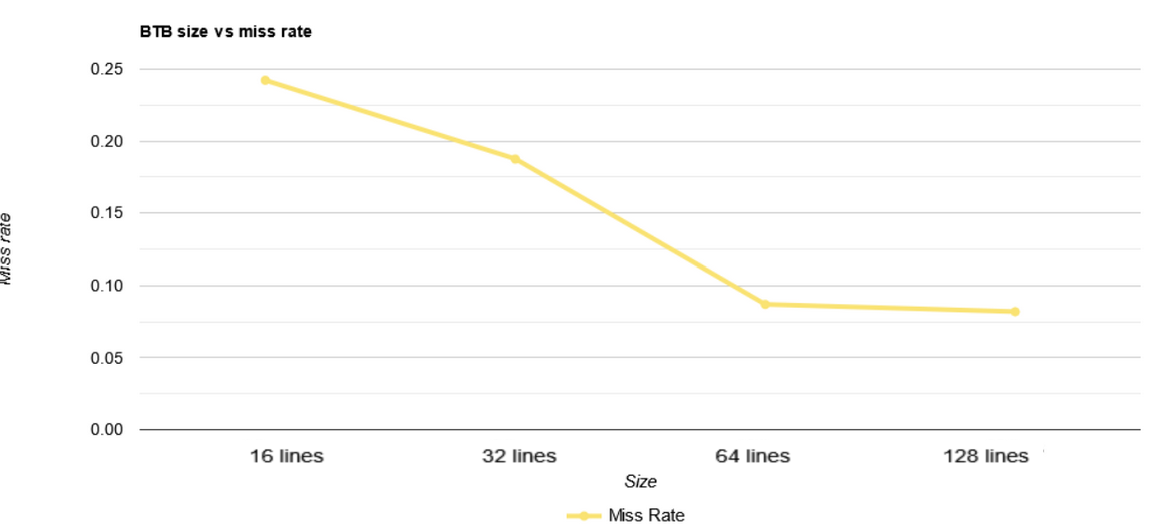
\includegraphics[width=0.5\textwidth]{figures/btb_missrate.png} % Replace with your image filename
    \caption{Relationship between btb size and miss rate on short programs.}
    \label{fig:sample-figure}
\end{figure}

\subsubsection{Direct-Mapped vs 4-Way Set Associative BTB}

Next, we compared a direct-mapped(DM) BTB and a 4-way set-associative(4-way SA) BTB, ensuring both have the same total number of entries (32). The associative BTB significantly reduces miss rate by mitigating conflicts.

\begin{center}
\textit{NM: Normalized}
\par\medskip
\begin{tabular}{|c|c|}
\hline
\textbf{BTB Configuration} & \textbf{Miss Rate}  \\
\hline
DM (32 lines) & 0.1876  \\
4-Way SA (8 sets) & 0.0686  \\
\hline
\end{tabular}
\end{center}

However, there is no significant CPI improvement on short programs, except for sort\_search.c.
\subsubsection{Round-Robin vs LRU Eviction Policies}

For set-associative BTBs, we explored two eviction strategies: Round-Robin and Least Recently Used (LRU). The main difference lies in whether the "used" bit is updated upon access.

\begin{center}
\begin{tabular}{|c|c|}
\hline
\textbf{Eviction Policy} & \textbf{Miss Rate} \\
\hline
Round-Robin & 0.0687  \\
LRU & 0.0686 \\
\hline
\end{tabular}
\end{center}

The results suggest that while LRU slightly outperforms Round-Robin, the difference is negligible in practice, especially considering the added complexity of tracking LRU.

\subsubsection{Hot Loading (Warm-Up Phase)}

Inspired by the idea of branch prediction warm-up, we implemented a "hot loading" strategy. We first ran the program once to collect BTB entries and then constructed a synthetic BTB to preload during program startup. This method aims to approximate a well-warmed-up BTB from the beginning of execution.

\begin{center}
\begin{tabular}{|c|c|}
\hline
\textbf{BTB State} & \textbf{Miss Rate} \\
\hline
No Warm-Up & 0.0686 \\
Hot-Loaded BTB & 0.0647 \\
\hline
\end{tabular}
\end{center}

This approach yielded a small yet consistent improvement, especially in short-running programs where warm-up matters more.

\subsubsection{Integration with Branch History}

To address the issue where the same branch address may lead to different targets (e.g., due to function pointers), we experimented with augmenting the BTB with branch history. We used both 2-bit and 3-bit global history mechanisms, applied to direct-mapped BTBs.

\begin{center}
\begin{tabular}{|c|c|}
\hline
\textbf{BTB Configuration} & \textbf{Miss Rate} \\
\hline
Direct-Mapped Only & 0.1876 \\
Direct-Mapped + 2-bit History & 0.1878 \\
Direct-Mapped + 3-bit History & 0.1924 \\
\hline
\end{tabular}
\end{center}

Unfortunately, incorporating short branch histories did not yield performance gains in our setup. We suspect that the history length was insufficient to capture meaningful patterns or that target aliasing was minimal in our benchmarks.



\section{Test}
\subsection{Unit Test}
\label{sec:rob-unittests}

We developed a comprehensive suite of fine-grained unit tests to validate all critical modules, such as the ROB and caches. In addition to testing basic functionalities, we specifically focus on edge cases. For instance, we designed our ROB test program to trigger branch resolution just as the ROB is nearing full capacity. By stressing these edge cases, we are able to identify potential bugs early in the process.

\subsection{Integrated Testing}

Initially, we tested our processor using default settings across all programs. To stress the processor further, we enabled various compiler optimization flags on the existing test programs. Specifically, we tested with the \texttt{-O1}, \texttt{-O2}, \texttt{-O3}, \texttt{-Ofast}, and \texttt{-Os} flags, and in all cases, the processor functioned correctly.

\subsection{Automated Testing}

To uncover potential issues more effectively, we designed simulators at different levels. These simulators not only allowed us to verify the correctness of every bit in all registers across all cycles but also enabled efficient identification of potential problems. For unit testing, we created simulators for more complex modules, such as the reservation station, and employed large random test cases to validate their correctness. 

As we integrated different modules, we transitioned to a C++-based, cycle-accurate simulator that precisely mimics the behavior of our SystemVerilog code. C++ allowed us to express certain logic more naturally. For instance, when selecting multiple candidates, we often need to check dependencies—such as ensuring that two branch instructions aren't fetched due to limitations in the prediction unit. This logic, which would require careful checking and complex selection in SystemVerilog, could be easily expressed as a \texttt{for} loop in C++. Additionally, C++ made it simpler to add extra checking logic and track multiple states, significantly enhancing our testing and debugging processes during the early stages.

The simulator is available in the "Simulator" folder on the "simulator" branch. However, it's important to note that the memory component is not yet fully implemented, so the simulator currently only works for programs without memory access.

\section{Project Management}

For Milestone 1, we focused on designing the layout of our processor. We chose the MIPS R10k architecture with a 2-way set-associative cache and the EBR feature. As part of this milestone, we prioritized the development of the Reservation Station (RS), the map table, and the Reorder Buffer (ROB) logic, as these components are foundational for several critical stages. We successfully completed all of these goals by the deadline, and in parallel, we designed the basic logic for the dispatch stage, which influences all subsequent stages.

For Milestone 2, we added early tag broadcasting to our plan while also working on the issue and completing the logic. Given the manageable workload, we aimed to deliver a functional processor (excluding memory operations). Additionally, we recognized the importance of creating a simulator for efficient debugging. We met all of these goals, though there was a one-day delay in completing the execute and complete stages.

Milestone 3 was primarily focused on the memory stage. After evaluating our tasks, we decided to implement a store queue and allow out-of-order memory access. We chose not to issue load instructions speculatively, as we felt this would complicate debugging. We also added several advanced performance features, including G-Share, a Return Address Stack (RAS), instruction prefetching, and a non-blocking data cache. While we completed these tasks by the deadline, we failed to identify a few bugs at that point, which were later uncovered during the integrated testing and optimization phase leading up to the final submission.

Before the final submission, our efforts were primarily focused on debugging and optimization. We reviewed parameter choices, which significantly improved both performance and reliability. Additionally, we began preparing for the presentation and report by gathering data and creating diagrams.

Throughout the process, our team worked collaboratively. In the beginning, we met frequently as a full group to discuss and code together. As the project progressed and tasks became more specialized, we divided into smaller groups of two to tackle specific modules (often one for implementation and the other working on testing), increasing our "group-level parallelism" (GLP). We synchronized our progress during larger group meetings, which allowed for greater parallelism and improved efficiency. By the time we reached the optimization stage, each team member focused on a specific task—whether it was identifying structural hazards, testing, or fine-tuning individual modules.

Assigned tasks are listed as follows:

\begin{itemize}
    \item Ding: load queue design and implementation; d-cache optimization
    \item Hu: functional units; cdb; store queue; connecting memory module with other parts
    \item Liu: debugging tools; parameter sweeping
    \item Song: branch target buffer optimization
    \item Yu: overall design; cache design and implementation; front-end; dispatch; issue
    \item Zhang: map table, free list, and branch predictor
\end{itemize}

Every group member is also responsible for testing several modules implemented by others.


\section*{Acknowledgment}

We gratefully acknowledge Professor Ron and Professor Kris for their invaluable guidance throughout this project. Our thanks also go to GSIs Bradley, Mustafa, and Jonah, as well as IA Gabby and IA Jaccob, for their thoughtful feedback, hands-on support in design and testing, and steadfast assistance with verification and the SystemVerilog toolchain. Your collective expertise and encouragement were essential to bringing this work to fruition.

\appendix

\section{Additional Results}

\begin{figure}[ht]
  \centering
  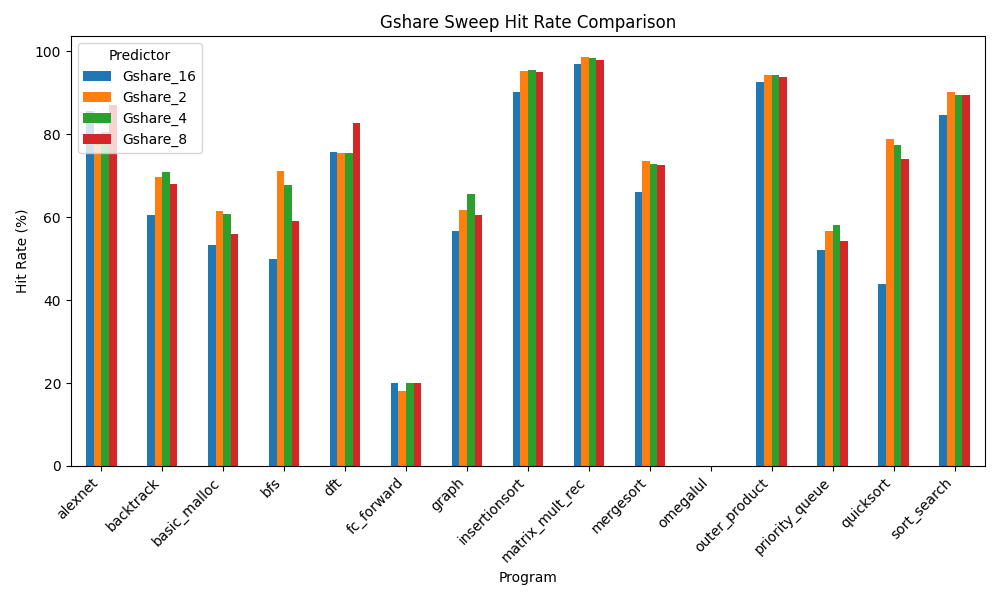
\includegraphics[width=0.35\textwidth]{figures/Appendix/gshare_sweep_bar.png}
  \caption{Comparison result of different BHR sizes of Gshare.}
  \label{fig:gshare-bhr}
\end{figure}

\begin{figure}[ht]
  \centering
  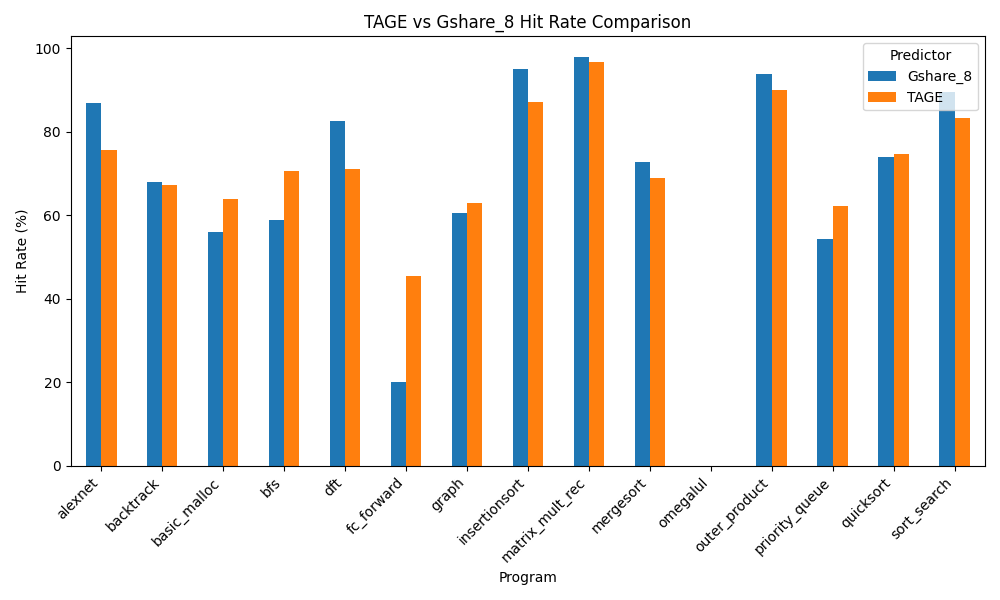
\includegraphics[width=0.35\textwidth]{figures/Appendix/tage_vs_gshare8_bar.png}
  \caption{Comparison between baseline (Gshare\_8) and TAGE.}
  \label{fig:gshare-tage}
\end{figure}

\begin{figure}[ht]
  \centering
  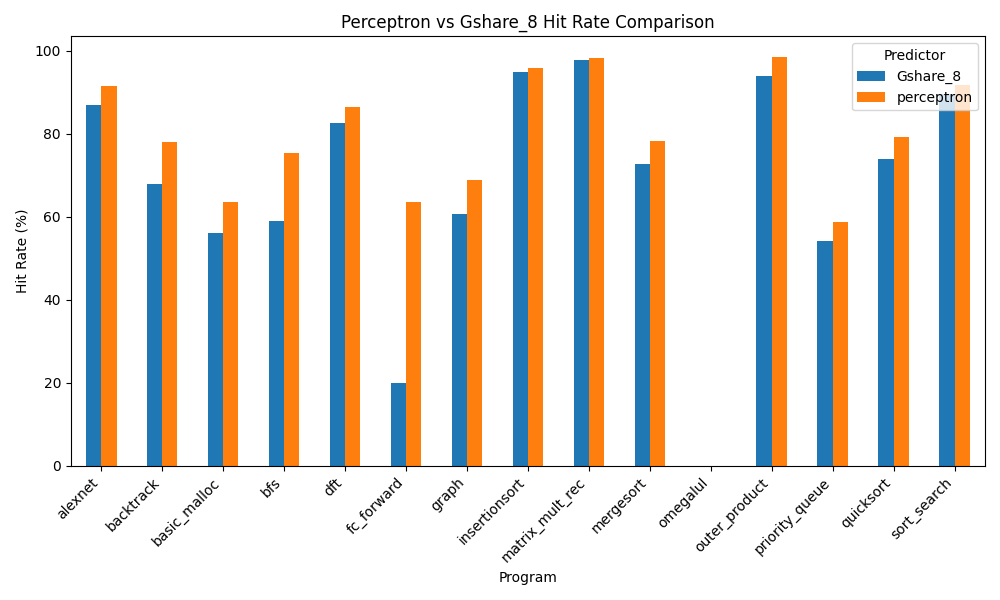
\includegraphics[width=0.35\textwidth]{figures/Appendix/Perceptron_vs_gshare8_bar.png}
  \caption{Comparison between baseline (Gshare\_8) and Perceptron.}
  \label{fig:gshare-perceptron}
\end{figure}

\begin{figure}[ht]
  \centering
  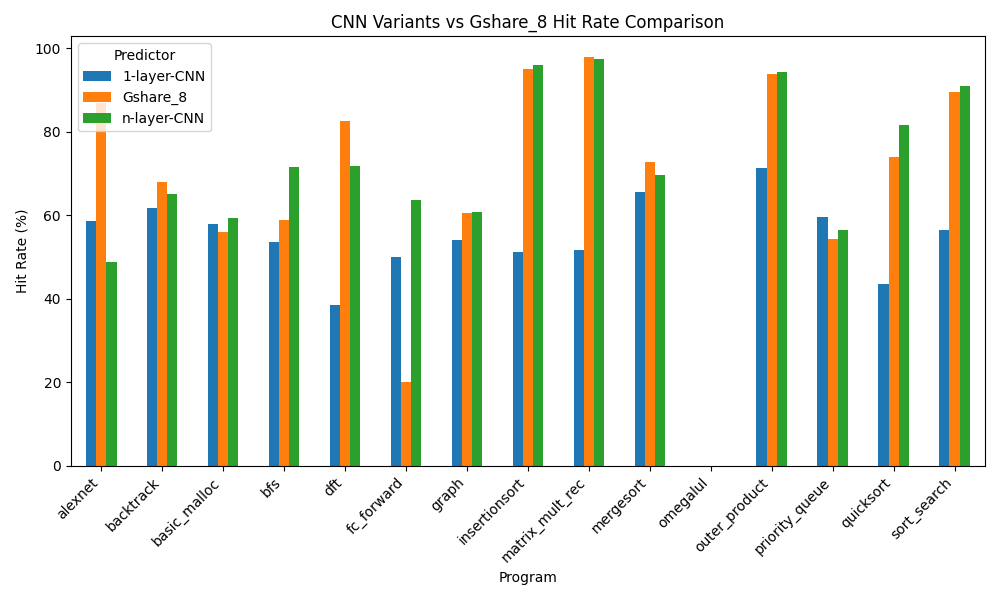
\includegraphics[width=0.35\textwidth]{figures/Appendix/cnn_vs_gshare8_bar.png}
  \caption{Comparison between baseline (Gshare\_8) and CNN.}
  \label{fig:gshare-cnn}
  \vspace{-10pt} 
\end{figure}

\end{document}
